\documentclass[10pt,twocolumn]{article}
\IfFileExists{lmodern.sty}{\usepackage{lmodern}}{}
\usepackage{amssymb,amsmath}
\usepackage{ifxetex,ifluatex}
\IfFileExists{fixltx2e.sty}{\usepackage{fixltx2e}}{} % provides \textsubscript on older LaTeX
\ifnum0\ifxetex1\fi\ifluatex1\fi=0% if pdftex
  \usepackage[T1]{fontenc}
  \usepackage[utf8]{inputenc}
\else % if luatex or xelatex
  \ifxetex%
    \usepackage{mathspec}
    \usepackage{xltxtra,xunicode}
  \else
    \usepackage{fontspec}
  \fi
  \defaultfontfeatures{Mapping=tex-text,Scale=MatchLowercase}
  \newcommand{\euro}{EUR}
\fi
% use upquote if available, for straight quotes in verbatim environments
\IfFileExists{upquote.sty}{\usepackage{upquote}}{}
% use microtype if available
\IfFileExists{microtype.sty}{\usepackage{microtype}}{}
\IfFileExists{geometry.sty}{\usepackage[letterpaper,top=0.8in,bottom=0.9in,left=0.75in,right=0.75in]{geometry}}{}
\usepackage{array,tabularx,booktabs}
\usepackage{graphicx}
\ifxetex%
  \usepackage[setpagesize=false, % page size defined by xetex
              unicode=false, % unicode breaks when used with xetex
              xetex]{hyperref}
\else
  \usepackage[unicode=true]{hyperref}
\fi
\hypersetup{breaklinks=true,
            bookmarks=true,
            pdfauthor={Tyler Baumgartner, Brandon Tai, Lisa Kaelin-Martin, Luc Debaupte, Bill Wang, Yi Zhong},
            pdftitle={VoiceCodeBench: Evaluating Exact Structured-Token Recovery in Automatic Speech Recognition},
            colorlinks=true,
            citecolor=blue,
            urlcolor=blue,
            linkcolor=magenta,
            pdfborder={0 0 0}}
\urlstyle{same}  % don't use monospace font for urls
\setlength{\parindent}{10pt}
\setlength{\parskip}{0pt}
\setlength{\emergencystretch}{3em}  % prevent overfull lines
\setcounter{secnumdepth}{0}
\setlength{\tabcolsep}{3pt}
\setlength{\columnsep}{0.25in}
\renewcommand{\arraystretch}{1.08}
\newcolumntype{L}{>{\raggedright\arraybackslash}X}

\title{VoiceCodeBench: Evaluating Exact Structured-Token Recovery in Automatic Speech Recognition}
\author{Tyler Baumgartner, Brandon Tai, Lisa Kaelin-Martin, Candice Fan,\\
Luc Debaupte, Bill Wang, and Yi Zhong\\
Besimple AI, San Mateo, CA\\
\texttt{\{tyler,yi\}@besimple.ai}}
\date{}


\begin{document}

\maketitle

\begin{abstract}

	Automatic speech recognition (ASR) systems are commonly evaluated with word
	error rate (WER), yet many voice workflows depend on exact written
	values for key entities. A transcript can appear fluent and achieve low WER
	while corrupting an identifier, path, or measured quantity that a
	downstream system must parse or store. When building voice agents, these 
	errors are not merely transcription defects. They can become wrong tool 
	arguments, invalid database fields, misrouted requests, or unsafe commands 
	while the transcript still looks plausible.

	We introduce \textbf{VoiceCodeBench}, a benchmark for evaluating exact
	structured-token recovery in English ASR\@. VoiceCodeBench contains 300
	human-recorded workplace segments across eight workflow domains and
	1,482 audited target entities across 26 entity types, each with a
	canonical written form recoverable from the spoken evidence.

	VoiceCodeBench uses a raw-audio-only evaluation protocol. Systems
	receive only audio bytes, with no additional context or metadata. Alongside
	WER, we introduce entity-sensitive measures, including Canonical
	Token/Entity Match (CTEM), Task Success Rate (TSR), and per-type exact
	recovery, to compare broad transcript accuracy with exact recovery of
	workflow-critical values.

	Across 12 baseline ASR systems, lower WER generally corresponded to better
	structured-token recovery, but it did not fully determine it: Spearman
	correlation was -0.73 between WER and CTEM and -0.73 between WER and TSR\@.
	Even the strongest baseline ASR system by TSR reached only 68.7\% TSR,
	meaning that nearly one third of recordings still contained at least
	one unrecovered workflow-critical value. These results show that WER is
	an informative transcript-quality diagnostic, but entity-sensitive
	metrics are needed to measure whether ASR output preserves the
	identifiers, commands, paths, measurements, and other exact values that
	production systems must parse, route, store, compare, or execute.
\end{abstract}

\section{Introduction}\label{introduction}

Speech interfaces increasingly mediate workflows that require exact
written values, such as contact details, file paths, account numbers,
and measured quantities. In such settings, a transcript is not only a
readable approximation of speech. It is software input that may be
stored, routed, compared, or executed. A sentence can look fluent while
still being unusable for the application that consumes it.

This creates a mismatch between common automatic speech recognition
(ASR) evaluation and production requirements. Word error rate (WER)
remains the standard summary metric for broad transcription quality
(National Institute of Standards and Technology, 2021), but it treats
word-level edits largely as interchangeable. A missing article can
count much like a corrupted structured value, even though only the latter
may misroute a support request, populate a record with the wrong
identifier, apply the wrong amount or unit, or execute the wrong tool
call. For structured tokens, punctuation, casing, separators,
token boundaries, digits, and spoken-to-written normalization can be part
of the value itself. A low-WER transcript can therefore be readable to a
person and still unsafe for the software system that consumes it.

Existing ASR benchmarks make broad progress measurable across many
sources of difficulty. LibriSpeech standardizes read audiobook speech,
Common Voice broadens speaker/language coverage through crowdsourcing,
GigaSpeech scales English ASR across web domains, FLEURS emphasizes
multilingual transfer, and AMI captures multi-party meeting speech
(Panayotov et al., 2015; Ardila et al., 2020; Chen et al., 2021;
Conneau et al., 2022; Carletta, 2007). These resources support
measurement of acoustic robustness, domain and language generalization,
and conversational transcription. A parallel line of work connects ASR
quality to meaning and application utility, including
spoken-language understanding accuracy, semantic distance, downstream
usability, named-entity recognition over ASR transcripts, and contextual
ASR (Wang et al., 2003; Kim et al., 2021; Roy, 2021; Szymanski et al.,
2023; Wang et al., 2025). However, these evaluations usually make
transcript fidelity, semantic similarity, named-entity recognition, or
context use the primary target. They do not directly answer a narrower
production question: given raw audio alone, did the ASR output preserve
enough evidence for every workflow-critical written value to be recovered
exactly?

VoiceCodeBench extends this foundation by making exact written-value
recoverability the unit of analysis. The benchmark focuses on ordinary
workplace domains where structured values are often the purpose of the
voice interaction rather than incidental edge cases. It is constructed
entity-first, with target entities allocated before transcripts are
written, producing controlled coverage by type, domain, and difficulty.
Each entity has a canonical written form recoverable from the acoustic
evidence, so evaluation can ask whether the transcript preserves the
specific value that an application would need to store, route, compare,
or execute.

VoiceCodeBench contains 300 human-recorded English workplace segments
with 1,482 target entities across 26 entity types and eight domains.
Under its raw-audio-only protocol, 12 ASR systems receive audio bytes
without target entities, domain labels, candidate values, prompts, custom
vocabulary, or other metadata. WER is reported alongside Canonical
Token/Entity Match (CTEM), Task Success Rate (TSR), and per-type exact
recovery. These metrics make different deployment questions visible.
WER measures broad transcript quality, CTEM measures value-level recovery
load, TSR measures whether a full segment can pass through an automated
workflow without repair, and per-type recovery identifies which classes
need safeguards such as confirmation prompts, constrained decoding, or
post-ASR validation. The benchmark therefore tests not only whether ASR
output reads well, but whether it preserves the exact values on which
workflow correctness depends.

\section{Methods}\label{methods}

\subsection{Benchmark Design}\label{benchmark-design}

VoiceCodeBench is designed as a test-only benchmark for evaluating
exact structured-token recovery in automatic speech recognition (ASR).
Each benchmark item contains a human-recorded English audio segment, a
reference transcript, item metadata including speaker and audio-quality
fields, and a set of target entities whose canonical written forms are
recoverable from their spoken form. The benchmark focuses on compact
workplace-style utterances containing values that downstream
applications may parse, route, store, compare, or execute.

During evaluation, ASR systems receive only the audio file
at inference time. This scope reflects a common pattern where
developers submit audio to an ASR provider and use the returned
transcript directly or with lightweight downstream processing.

The dataset contains 300 human-recorded English segments
across eight workflow domains, summarized in
Table~\ref{tab:workflow-domains}. The domain distribution is not
intended as an estimate of how often these workflows occur in
production speech. It is designed to provide enough examples of each
structured-token failure mode for per-type analysis.

\begin{table*}[t]\centering\footnotesize
	\caption{Workflow-domain distribution.}\label{tab:workflow-domains}
	\begin{tabularx}{\textwidth}{lrL}
		\toprule
		Domain                     & Recordings & Purpose
		\\
		\midrule
		Contact/routing            & 45         & Callback numbers, extensions, emails, postal
		addresses, spelled names, routing teams
		\\
		Technical/IT/dev           & 55         & Commands, flags, files, URLs, IPs, ports,
		versions, symbols, environment variables
		\\
		Retail/logistics/order     & 45         & SKUs, serials, tracking IDs, quantities,
		addresses, returns, subscriptions
		\\
		Finance/billing            & 40         & Invoices, account numbers, currency, percentages,
		rates, dates, payment details
		\\
		Healthcare/admin           & 35         & Appointments, measurements, dosages, record
		numbers, referrals, insurance terms
		\\
		Legal/insurance/government & 35         & Claims, policies, case IDs, exhibit
		labels, formal references, addresses
		\\
		Education/workplace        & 25         & HR, courses, rooms, employee IDs, internal
		helpdesk, facilities
		\\
		Dense mixed stress         & 20         & High entity load and cross-type interference
		under compact spoken conditions
		\\
		\bottomrule
	\end{tabularx}\end{table*}

The benchmark includes 1,482 target entities across 26 entity types,
with an average of 4.94 target entities per recording. Gold acoustic
transcript lengths range from 95 to 206 words depending on difficulty
band. Each recording is assigned a difficulty band that combines entity load,
entity complexity, transcript length, and expected recovery challenge.
Table~\ref{tab:difficulty-bands} summarizes the band design.

\begin{table}[t]\centering\footnotesize
	\caption{Difficulty-band design.}\label{tab:difficulty-bands}
	\begin{tabular}{lrll}
		\toprule
		Difficulty & Recordings & Entity load   & Acoustic transcript length
		\\
		\midrule
		Light      & 30         & 3 entities    & 95--130 words
		\\
		Standard   & 114        & 4 entities    & 103--169 words
		\\
		Dense      & 93         & 5--6 entities & 122--177 words
		\\
		Stress     & 63         & 7--8 entities & 156--206 words
		\\
		\bottomrule
	\end{tabular}\end{table}

All scenarios and structured values are synthetic. The
\hyperref[ethical-and-privacy-considerations]{Ethical and Privacy
Considerations section} describes the privacy constraints used when
constructing these values.

VoiceCodeBench organizes target entities by recovery behavior rather
than by workflow domain alone. The taxonomy contains 26 entity types
grouped into six broad categories (Table~\ref{tab:entity-taxonomy}).

\begin{table*}[t]\centering\footnotesize
	\caption{Entity taxonomy used for structured-token scoring.}\label{tab:entity-taxonomy}
	\begin{tabularx}{\textwidth}{lL}
		\toprule
		Group                   & Entity types
		\\
		\midrule
		Contact and routing     & \texttt{email\_address}, \texttt{phone\_number},
		\texttt{phone\_extension}, \texttt{person\_or\_team\_name},
		\texttt{postal\_address}
		\\
		Network and web         & \texttt{url}, \texttt{ip\_address},
		\texttt{port\_number}
		\\
		Code and system         & \texttt{command}, \texttt{cli\_flag},
		\texttt{file\_path}, \texttt{environment\_variable},
		\texttt{code\_symbol}, \texttt{version}
		\\
		Identifiers             & \texttt{reference\_id}, \texttt{product\_code},
		\texttt{account\_or\_record\_number}
		\\
		Numeric and measurement & \texttt{currency\_amount},
		\texttt{percentage}, \texttt{measurement}, \texttt{plain\_number},
		\texttt{date}, \texttt{time}
		\\
		Language form           & \texttt{acronym\_or\_initialism},
		\texttt{spelled\_sequence}, \texttt{domain\_term}
		\\
		\bottomrule
	\end{tabularx}\end{table*}

The taxonomy captures values that are both exactness-sensitive and critical to
real-world ASR-backed production workflows. Some entities, such as phone 
numbers or dates, may be recoverable under conventional formatting 
normalization. Others, such as file paths or command-line flags, treat 
punctuation and separators as part of the value itself.

VoiceCodeBench is not intended as a general-purpose ASR corpus or a
training set. It is released as a diagnostic evaluation resource.

\subsection{Entity and Transcript
	Generation}\label{entity-transcript-generation}

VoiceCodeBench was constructed entity-first. For each item, we first
specified the workflow domain, difficulty band, target entity count,
and target entity types. We then generated unique synthetic entities for
the required slots, assigned each value both an acoustic form and a
canonical form. Finally, we wrote a workplace-style transcript around
that planned entity bundle. This ordering prevents the dataset from
merely extracting whichever structured values happen to appear in
free-form scripts, and it allows coverage to be controlled across
entity types, workflow domains, and difficulty bands.

Generation was LLM-assisted but constraint-driven. We used a
repository-aware LLM workflow to draft and check items under fixed
metadata, entity, and validation constraints. Implementation details are
provided in \hyperref[appendix-generation-tooling]{the generation-tooling
	appendix}. This workflow helped maintain the benchmark
metadata structure, populate the template, acoustic, and canonical
transcript layers, and enforce the requested domain, difficulty, and
entity-type constraints. Candidate items were accepted only after
validation and review for domain fit, naturalness, uniqueness, entity
consistency, and recoverability.

The acoustic form represents what the speaker is expected to say. It
may include spoken symbols, spelling cues, casing instructions, or
formatting instructions. The canonical form represents the exact written
value that a downstream application must recover. This distinction makes
explicit the gap between what is said and what software needs to
consume.

\[
	\begin{array}{@{}rcl@{}}
		\text{\footnotesize ``double dash dry dash run''}         & \rightarrow &
		\text{\footnotesize\texttt{-\kern0pt-dry-run}}                                  \\
		\text{\footnotesize ``all caps database underscore URL''} & \rightarrow &
		\text{\footnotesize\texttt{DATABASE\_URL}}
	\end{array}
\]

The acoustic form alone must provide enough information for a careful
listener to infer the intended canonical value. An entity is rejected or
revised if its canonical value is not uniquely recoverable from the
intended acoustic form. For example, a target requiring
\texttt{DATABASE\_URL} must include sufficient spoken evidence for the
underscore and casing convention.

The scenarios and structured values are synthetic, while the released
audio is human-recorded. Synthetic content avoids exposing real contact
details, accounts, credentials, or operational systems. Email addresses
and URLs use reserved documentation domains and controlled domains.
Phone numbers use fictional NANP \texttt{555\mbox{-}0100} through
\texttt{555\mbox{-}0199} numbers with varied area codes. Public-looking IPv4
addresses use documentation ranges, while internal network examples use
private address ranges. Postal addresses, account numbers, product
codes, reference IDs, and workflow scenarios are synthetic.

The dataset may include public organization, product, or platform names
when they function as ordinary workplace vocabulary, but these names are
not paired with real private contact records or live routable
information. This allows the benchmark to test recognition of common
workplace terms while keeping sensitive fields synthetic or reserved.

\subsection{Recording and Verification}\label{recording-verification}

Each transcript is recorded by a human speaker reading one compact
workplace-style segment. Speakers read the acoustic transcript layer,
which renders target entities in the form intended to be spoken rather
than as their canonical scoring values. Speakers are instructed to read
naturally but clearly, preserving dictated punctuation phrases, spelling
sequences, casing cues, and formatting instructions. The intended style is
deliberate workplace dictation rather than theatrical performance or
casual conversation.

Recordings are collected remotely through a crowdsourcing platform from
paid contributors who consent to dataset use and release. After recording,
each audio file is human audited. Files with severe audio quality
issues or that contain spoken errors are rejected and re-recorded.
Accepted audio files are released without additional post-processing.

\subsection{Transcription Protocol}\label{transcription-protocol}

All ASR systems receive only the raw audio file for each
recording. Batch systems transcribe each complete file; streaming systems
receive chronological audio chunks under a fixed chunking policy. Only final
transcripts are scored. Provider defaults are used except for settings
needed to select the intended model or English language mode. Provider
punctuation, capitalization, and formatting are allowed, but benchmark-
specific prompting, custom vocabulary, entity hints, grammar constraints,
and post-ASR correction are excluded from the main raw-audio-only evaluation.
For each baseline ASR system, we record the provider, model, endpoint or API, batch or
streaming mode, evaluation date, and reproduction-relevant inference settings.

\subsection{Entity Extraction}\label{entity-extraction}

Entity extraction asks whether each gold canonical value is recoverable
from the ASR transcript. Formatting variation is accepted when it preserves 
the same value, such as a phone number rendered as an uninterrupted digit 
sequence or a currency amount rendered as an unambiguous spoken amount. 
Separators, casing cues, units, digits, token boundaries, and punctuation are 
treated as value-bearing when they determine the canonical string, as in email 
addresses, file paths, URLs, environment variables, code symbols, and command-line 
flags.

The entity extraction policy is applied with an LLM-powered recoverability
verifier. The verifier receives the ASR transcript and the target entities,
including type, acoustic form, and canonical form, and returns strict JSON
with one result per target index, including type, canonical value, present/absent 
decision, evidence span, and reason. It is instructed to mark an entity
present only when the transcript contains enough evidence to recover the exact
canonical value, and to reject wrong, missing, extra, or substituted letters,
digits, separators, units, dates, times, amounts, or words that change the
value. The tracked verifier is the versioned artifact
\texttt{openai\_gpt\_5\_5\_v1}, using \texttt{GPT-5.5}. The full verifier
system prompt is provided in
\hyperref[appendix-verifier-prompt]{the verifier-prompt appendix}. Verifier
outputs include evidence and reasons, and edge cases
identified during baseline analysis were manually reviewed. As a reliability
check, a human auditor reviewed a stratified sample of 200 entity decisions
across ASR models and entity types. Agreement with the verifier decisions was
100\%. The reviewed rows are released as
\texttt{audit/verifier\_audit\_samples.csv}.

\subsection{Metrics and Scoring}\label{metrics}\label{statistical-reporting}\label{baseline-systems}

VoiceCodeBench includes WER as a broad transcript-accuracy comparison
and reports entity-sensitive metrics for workflow-critical value
recovery. WER compares the model transcript with the gold acoustic
transcript after both strings are lowercased and reduced to word tokens.
Punctuation and separators are not scored as standalone WER tokens.

The primary entity metric is Canonical Token/Entity Match:

\[
	\mathrm{CTEM} =
	\frac{N_{\mathrm{correct\ entities}}}{N_{\mathrm{target\ entities}}}
\]

CTEM is measured overall and by entity type, workflow domain, difficulty
band, and evaluation mode. Task Success Rate measures whether all target
entities in a recording are recovered correctly:

\[
	\mathrm{TSR} =
	\frac{N_{\mathrm{successful\ recordings}}}{N_{\mathrm{recordings}}}
\]

TSR is intentionally strict. Many workflow segments are not safe to use
in production settings if even one required value is corrupted. Overall
confidence intervals are calculated using Wilson 95\% binomial intervals.
Slice tables are reported as descriptive baseline summaries without
confidence intervals.

VoiceCodeBench evaluates both commercial and open ASR systems in batch
and streaming settings. The baseline suite covers ASR systems from
major commercial providers and open models under the raw-audio-only
protocol described above. Table~\ref{tab:baseline-systems} lists the
baseline ASR systems used in the benchmark.

\begin{table*}[t]\centering\footnotesize\begin{tabular}{llc}
		\toprule
		Provider          & Model                       & Mode
		\\
		\midrule
		Deepgram          & Nova-3                      & Batch
		\\
		OpenAI            & GPT-4o Transcribe           & Batch
		\\
		AssemblyAI        & Universal-3 Pro             & Batch
		\\
		Google Cloud      & Chirp 3                     & Batch
		\\
		ElevenLabs        & Scribe v2                   & Batch
		\\
		Groq              & Whisper Large v3            & Batch
		\\
		Amazon Transcribe & Amazon Transcribe Streaming & Streaming
		\\
		Deepgram          & Nova-3                      & Streaming
		\\
		OpenAI            & GPT Realtime Whisper        & Streaming
		\\
		AssemblyAI        & Universal-3 Pro             & Streaming
		\\
		Google Cloud      & Chirp 3                     & Streaming
		\\
		ElevenLabs        & Scribe v2 Realtime          & Streaming
		\\
		\bottomrule
	\end{tabular}
	\caption{Baseline ASR systems evaluated by VoiceCodeBench.}\label{tab:baseline-systems}
\end{table*}

\section{Results}\label{results}

\subsection{Dataset Composition}\label{dataset-composition}

The completed baseline release evaluates the 300-recording benchmark
described in Methods. The evaluated audio totals 5.58 hours from 85
unique speakers, and the baseline suite contains 12 baseline ASR systems.

The target-entity distribution is intentionally broad. Entity types such
as reference IDs, product codes, dates, acronyms, and spelled sequences
appear frequently, while lower-frequency but operationally important
classes such as file paths, environment variables, port numbers,
percentages, and measurements are explicitly represented.
Table~\ref{tab:entity-counts} reports the target-entity counts by type.

\begin{table*}[t]\centering\footnotesize
	\caption{Target-entity counts by entity type.}\label{tab:entity-counts}
	\begin{tabularx}{\textwidth}{LrLrLr}
		\toprule
		Entity type                          & Count & Entity type              & Count & Entity type                     & Count
		\\
		\midrule
		\texttt{reference\_id}               & 150   & \texttt{url}             & 62    & \texttt{code\_symbol}           & 35
		\\
		\texttt{spelled\_sequence}           & 97    & \texttt{measurement}     & 61    & \texttt{environment\_variable}  & 35
		\\
		\texttt{product\_code}               & 90    & \texttt{phone\_number}   & 60    & \texttt{phone\_extension}       & 30
		\\
		\texttt{date}                        & 89    & \texttt{time}            & 60    & \texttt{port\_number}           & 30
		\\
		\texttt{acronym\_or\_initialism}     & 85    & \texttt{file\_path}      & 51    & \texttt{version}                & 30
		\\
		\texttt{currency\_amount}            & 75    & \texttt{command}         & 50    & \texttt{ip\_address}            & 25
		\\
		\texttt{account\_or\_record\_number} & 65    & \texttt{percentage}      & 50    & \texttt{domain\_term}           & 20
		\\
		\texttt{plain\_number}               & 65    & \texttt{cli\_flag}       & 44    & \texttt{person\_or\_team\_name} & 18
		\\
		\texttt{email\_address}              & 65    & \texttt{postal\_address} & 40    &                                 &
		\\
		\bottomrule
	\end{tabularx}\end{table*}

\subsection{Overall ASR and Structured-Token
	Performance}\label{overall-asr-and-structured-token-performance}

Table~\ref{tab:overall-results} reports overall performance for each
baseline ASR system. All scores are percentages.

\begin{table*}[t]
	\centering
	\footnotesize
	\setlength{\tabcolsep}{4.5pt}
	\begin{tabular*}{\textwidth}{@{\extracolsep{\fill}}l l r r c r c@{}}
		\toprule
		Model & Mode & WER $\downarrow$ & CTEM $\uparrow$ & CTEM 95\% CI & TSR $\uparrow$ & TSR 95\% CI
		\\
		\midrule
		ElevenLabs Scribe v2 & Batch & 16.1 & \textbf{91.6} & 90.0--92.9 & 67.7 & 62.2--72.7
		\\
		Deepgram Nova-3 & Batch & \textbf{8.6} & 90.9 & 89.3--92.3 & \textbf{68.7} & 63.2--73.7
		\\
		Deepgram Nova-3 & Streaming & 9.6 & 88.9 & 87.2--90.4 & 61.7 & 56.1--67.0
		\\
		Google Cloud Chirp 3 & Batch & 25.6 & 88.8 & 87.1--90.3 & 60.3 & 54.7--65.7
		\\
		OpenAI gpt-realtime-whisper & Streaming & 16.3 & 88.7 & 87.0--90.2 & 59.3 & 53.7--64.7
		\\
		Whisper large-v3 & Batch & 23.1 & 87.6 & 85.8--89.2 & 54.3 & 48.7--59.9
		\\
		OpenAI gpt-4o-transcribe & Batch & 24.6 & 87.4 & 85.6--89.0 & 55.7 & 50.0--61.2
		\\
		Google Cloud Chirp 3 & Streaming & 25.5 & 86.1 & 84.2--87.8 & 50.3 & 44.7--56.0
		\\
		AssemblyAI Universal-3 Pro & Batch & 25.2 & 84.5 & 82.6--86.3 & 50.3 & 44.7--56.0
		\\
		ElevenLabs Scribe v2 realtime & Streaming & 24.9 & 84.0 & 82.1--85.8 & 46.3 & 40.8--52.0
		\\
		AssemblyAI Universal-3 Pro & Streaming & 25.2 & 78.3 & 76.1--80.3 & 33.0 & 27.9--38.5
		\\
		Amazon Transcribe & Streaming & 25.6 & 75.2 & 73.0--77.4 & 33.7 & 28.6--39.2
		\\
		\bottomrule
	\end{tabular*}
	\caption{Overall baseline performance on 300 recordings and 1,482 target entities.}\label{tab:overall-results}
\end{table*}

Across baseline ASR systems, WER ranged from 8.6 to 25.6, while CTEM
ranged from 75.2 to 91.6 and TSR ranged from 33.0 to 68.7. The main
empirical result is that transcript-level accuracy and structured-token
recovery are correlated, but the association is incomplete.

To test whether ordinary transcript accuracy predicts structured-token
correctness, we compare WER against CTEM and TSR across systems
(Figure~\ref{fig:wer-entity-scatter}). WER has Spearman correlation
$\rho=-0.73$ with CTEM and $\rho=-0.73$ with TSR\@. The negative signs
reflect the opposite metric directions: lower WER is better, while
higher CTEM and TSR are better. The magnitudes indicate a strong
monotonic association, so WER is informative, but the spread in the
figure shows that it does not fully determine structured-token
correctness.

\begin{figure*}[t]\centering
	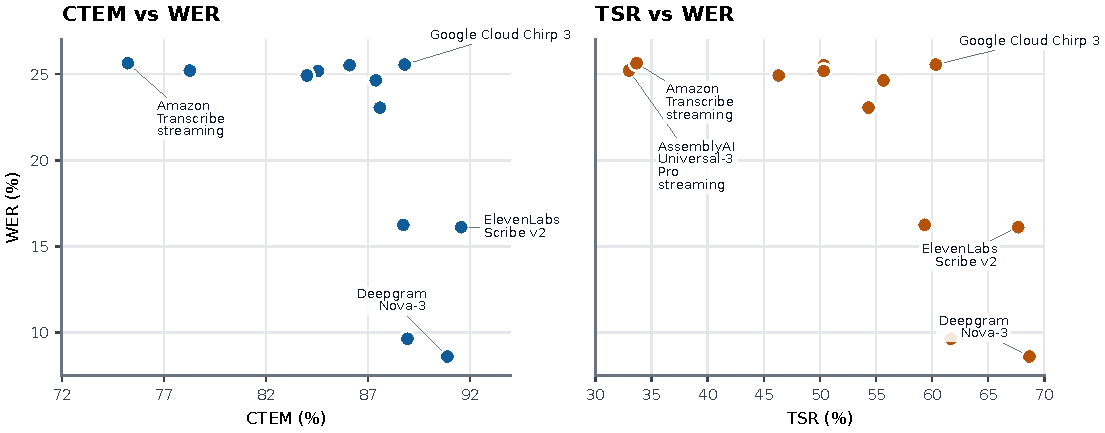
\includegraphics[width=0.86\textwidth]{figures/wer_entity_scatter.pdf}
	\begin{minipage}[t]{0.43\textwidth}\footnotesize
		\textbf{CTEM vs WER.} Spearman correlation is -0.73: lower WER
		generally tracks higher entity-level recovery, while substantial spread
		remains.
	\end{minipage}\hfill
	\begin{minipage}[t]{0.43\textwidth}\footnotesize
		\textbf{TSR vs WER.} Spearman correlation is -0.73: lower WER also
		tracks full workflow success, with a similar association to CTEM\@.
	\end{minipage}
	\caption{WER compared with entity-sensitive metrics across 12
		baseline ASR systems, with WER shown on the shared vertical axis. Each
		point is one baseline ASR system. The negative monotonic correlations show that ordinary
		transcript accuracy is related to structured-token recovery, while the
		spread of points shows that WER does not fully determine CTEM or TSR.}\label{fig:wer-entity-scatter}
\end{figure*}

\subsection{Performance by Entity
	Type}\label{performance-by-entity-type}

The evaluation artifacts contain 17,784 model-entity decisions across 12
baseline ASR systems, of which 2,489 are entity failures. These failures
are concentrated in punctuation- and boundary-sensitive classes: URLs,
commands, email addresses, file paths, and postal addresses account for
1,484 failures, or 59.6\% of all entity failures. Because raw failure
counts reflect both entity prevalence and entity difficulty, we treat
these counts descriptively; the per-type CTEM results in this section
are the main basis for comparing entity difficulty.

Entity-type results show that the hardest values are those whose written
forms depend on symbols, separators, and exact token boundaries. Median
CTEM is lowest for \texttt{command} (45.0), \texttt{url} (48.4),
\texttt{file\_path} (56.9), \texttt{postal\_address} (57.5), and
\texttt{email\_address} (65.4). In contrast, highly conventional
numeric forms such as \texttt{percentage}, \texttt{measurement},
\texttt{date}, and \texttt{plain\_number} are recovered reliably by
most systems. The same contrast appears in the taxonomy groups in
Table~\ref{tab:entity-taxonomy}, where numeric and measurement values and
language-form entities are high at 97.3 and 95.0 CTEM, while network/web
and code/system values trail at 68.7 and 69.4 because they concentrate
URLs, commands, file paths, flags, and environment variables. The largest
cross-model spreads occur for \texttt{url},
\texttt{command}, \texttt{file\_path}, and
\texttt{environment\_variable}, making these types especially useful
for differentiating ASR systems beyond WER\@. For the same reason,
domain-level aggregates are best read descriptively, since workflow
domains differ mainly in their entity mix. Appendix
Tables~\ref{tab:appendix-domain-performance} and
\ref{tab:appendix-difficulty-performance} provide descriptive domain and
difficulty slices for reference.

Table~\ref{tab:error-examples} shows representative cases extracted
from the baseline evaluations that illustrate the distinction between
\textbf{recoverable formatting variation} and \textbf{unrecoverable
	evidence loss}. Some transcripts omit canonical formatting while
preserving enough information to reconstruct the value. Others destroy
essential evidence, such as digits, symbols, separators, or units.
VoiceCodeBench counts the former as correct when the value remains
uniquely recoverable and the latter as incorrect.

\begin{table*}[t]\centering\footnotesize\begin{tabularx}{\textwidth}{LLLLL}
		\toprule
		Entity type                                     & Gold canonical                  & Transcript evidence     & Error class &
		Recoverable?
		\\
		\midrule
		\texttt{cli\_flag}                              & \texttt{-\kern0pt-dry-run}      & ``dry run''             & symbol loss &
		No
		\\
		\texttt{environment\_variable}                  & \texttt{DATABASE\_URL}          & ``database
		URL''                                           & underscore/casing loss          & No
		\\
		\texttt{phone\_number}                          & \texttt{212\mbox{-}555\mbox{-}0104} & ``two one two five five
		five zero one zero four''                       & formatting variation            & Yes
		\\
		\texttt{file\_path}                             & \texttt{/var/log/.\kern0pt.\kern0pt./error.log} & ``var log
		engine x error log''                            & path flattening / substitution  & No
		\\
		\texttt{currency\_amount}                       & \texttt{\$7,930.79}             & ``seven thousand nine
		hundred thirty dollars and seventy nine cents'' & formatting variation            &
		Yes
		\\
		\texttt{measurement}                            & \texttt{500 mg}                 & ``500 micrograms''      & unit error
		                                                & No
		\\
		\bottomrule
	\end{tabularx}\caption{Examples from the baseline evaluations illustrating recoverable and unrecoverable structured-token cases.}\label{tab:error-examples}\end{table*}

\section{Discussion}\label{discussion}

\subsection{Principal Findings}\label{principal-findings}

VoiceCodeBench is designed to measure a production failure mode that
is easy to miss with ordinary transcript-level evaluation. The central
empirical finding is that WER is useful but incomplete as a predictor of
application-facing ASR reliability. Across systems, lower WER generally
corresponded to better structured-token recovery, with Spearman
correlation $\rho=-0.73$ for CTEM and $\rho=-0.73$ for TSR in
Figure~\ref{fig:wer-entity-scatter}. That association means WER remains
informative. The spread across systems means it cannot stand in for
entity-level or workflow-level correctness. An ASR system can produce a
fluent, low-WER transcript while still corrupting the exact structured
values that make a workflow usable. The baseline results show that this
risk remains present even for strong modern ASR systems. The best TSR in
this release was 68.7\%, so nearly one third of recordings still
contained at least one unrecovered workflow-critical value.

The system with the lowest WER and highest TSR was Deepgram Nova-3
batch, while the highest CTEM came from ElevenLabs Scribe v2 batch. The
weakest structured-token performance appeared for Amazon Transcribe
streaming and AssemblyAI Universal-3 Pro streaming. Streaming usually
reduced CTEM and TSR relative to paired batch systems, with OpenAI as the
exception in this run. These rank differences are practically important. A
provider choice that looks best under WER is not necessarily the one
that minimizes value-level repair work, and a system that recovers many
individual entities can still fail full workflows when errors are spread
across recordings.

The most informative failures were not uniformly distributed. The largest
performance gaps occurred for URLs, commands, file paths, email
addresses, postal addresses, and environment variables. Apparent domain
differences largely followed where these entity types appeared. These
classes are particularly useful for differentiating systems because they
require preservation of symbols, separators, digit sequences, casing
cues, or token boundaries rather than only recognition of ordinary words.
This concentration is one of the benchmark's central findings. Exact
structured-token reliability depends on the written conventions of the
entity type, not only on the acoustic difficulty of the surrounding
sentence.

\subsection{What Entity-Sensitive Evaluation
	Reveals}\label{what-entity-sensitive-evaluation-reveals}

WER remains useful for measuring broad transcription quality, but
VoiceCodeBench shows why it is incomplete for application-facing
speech interfaces. Word-level edit distance can dilute the importance of
rare but critical values. A transcript may correctly recognize a long
surrounding sentence while losing the one value that the application
needs to parse, route, store, compare, or execute.

CTEM and TSR make this failure mode visible. CTEM asks whether each
target value remains recoverable from the transcript. TSR asks whether
the whole segment is safe for the corresponding workflow. Per-type
recovery identifies which value classes are fragile. Reporting these
metrics alongside WER allows us to distinguish three cases. These are
systems that are broadly accurate and preserve structured values,
systems that are broadly accurate but unreliable on structured values,
and systems that have both high transcript error and high
structured-token error.

This distinction changes how ASR results can be used by product and
platform teams. WER is appropriate for monitoring general transcript
quality, but CTEM estimates value-level correction burden, TSR estimates
the fraction of recordings that can flow through automation without
human or programmatic repair, and per-type recovery points to targeted
mitigations. A team building support routing, form filling, developer
tooling, healthcare administration, or billing workflows may therefore
choose different ASR settings, add confirmation for only certain entity
types, or reject an otherwise strong model if its failures cluster in
high-cost values. The correlation analysis reinforces this point. Lower
WER is associated with higher CTEM and TSR across systems, but the
relationship is not deterministic, so aggregate transcript accuracy can
hide weaknesses in specific entity classes.

\subsection{Punctuation and Normalization as
	Correctness}\label{punctuation-and-normalization-as-correctness}

A recurring theme in VoiceCodeBench is that punctuation, formatting,
and normalization are not merely cosmetic. In ordinary transcript
readability tasks, punctuation and capitalization may be treated as
presentation details or post-processing targets. In structured workflow
tokens, they can define the value itself. Dashes, dots, slashes,
underscores, equals signs, leading zeros, decimal points, units, and
token boundaries may determine whether a value is parseable and correct.

This is why the benchmark distinguishes between acoustic and canonical
forms. The acoustic form captures what the speaker said; the canonical
form captures what the application needs. The relevant question is not
whether the transcript exactly matches a reference sentence, but whether
it preserves enough evidence to recover the intended canonical value.
For example, a phone number may remain recoverable even if hyphens are
omitted, because the digit sequence is intact. By contrast, a file path
or email address may become unrecoverable if slashes, dots, or
separators are lost.

The baseline examples in Table~\ref{tab:error-examples} support this
distinction. Failures such as URL domain corruption, command
substitution, path segment loss, email-domain corruption, suite/unit
confusion, and environment-variable word-form substitution are not
merely formatting imperfections. They change the value available to
downstream software. This suggests that ASR evaluation for workflow use
should treat punctuation-sensitive and normalization-sensitive values as
first-class targets rather than as secondary presentation features.

\subsection{Intended Use}\label{intended-use}

VoiceCodeBench is intended as a diagnostic benchmark for
structured-token reliability in ASR systems. It supports provider
comparison, regression tracking, per-entity risk analysis, and decisions
about application-specific safeguards. Strong aggregate performance is
not sufficient when weak recovery for entities such as
\texttt{file\_path}, \texttt{email\_address}, or
\texttt{currency\_amount} may still require validation, confirmation
prompts, constrained decoding, or downstream repair before production
use.

The practical implication for applications like \textbf{voice agents} is that
transcript readability and low WER are insufficient deployment gates
when ASR output feeds tool calls, form fills, database writes, routing
logic, or command execution. Agent pipelines should evaluate whether the
specific values they act on remain recoverable, then pair ASR selection
with product controls such as confirmation prompts, typed validation,
constrained inputs, or human review for high-risk entity classes.

The benchmark is not a general measure of ASR quality, a training
corpus, a fine-tuning set, or a hidden leaderboard. It does not cover all
speech styles, languages, acoustic environments, or conversational
settings. Because labels are public, reports should disclose model
versions, evaluation dates, inference settings, and any
benchmark-specific prompting, post-processing, fine-tuning, or
canonicalization. Its best use is comparative and diagnostic, identifying
which systems preserve exact structured values, which entity types or
workflow slices are fragile, and which errors remain recoverable from
transcript evidence.

\subsection{Limitations}\label{limitations}

VoiceCodeBench is intentionally focused, and its results should be
interpreted within that scope. First, the benchmark is English-only.
Structured-token dictation is common in many languages, but punctuation
conventions, spelling practices, number formats, address formats, and
spoken symbol conventions vary across languages. Multilingual evaluation
will require additional design work rather than direct translation.

Second, the benchmark focuses on compact workplace-style dictation. It
does not attempt to cover all ASR conditions, including casual
conversation, meetings, overlapping speech, broadcast audio, voice
search, noisy field recordings, or long-form dictation. This narrowness
is deliberate because the benchmark targets a specific workflow failure
mode.
However, results should not be generalized to all speech-recognition use
cases.

Third, the scenarios and values are synthetic, even though the audio is
human-recorded. Synthetic content allows controlled coverage and safer
public release, but it may not capture every distributional property of
real support calls, developer conversations, clinical documentation,
logistics workflows, or financial operations. Some generated scenarios
may be cleaner or more compact than naturally occurring speech.

Fourth, exact structured-token scoring requires policy choices and
currently uses LLM-assisted recoverability verification. VoiceCodeBench
counts an entity as correct if the transcript contains enough evidence
to recover the canonical value exactly, even when that evidence appears
in spoken or partially normalized form. This is more flexible than
literal string match, but it requires careful handling of borderline
cases and introduces dependence on the verifier model and prompt. Some
values are clearly recoverable despite formatting variation; others
become ambiguous when symbols, separators, or units are omitted. The
benchmark mitigates this by documenting scoring rules, the verifier
artifact \texttt{openai\_gpt\_5\_5\_v1}, its model \texttt{gpt-5.5}, the
prompt, the strict JSON response schema, the absence of a temperature override
for GPT-5-family verifier models,
per-model verifier JSON files with evidence spans and reasons, and final
scoring files. A human audit of 200 entity decisions sampled across ASR
models and entity types found 100\% agreement with the verifier decisions.
Future versions should expand deterministic scoring for entity types where
exact canonicalization can be implemented reliably, but some edge cases will
remain debatable.

Fifth, commercial ASR systems change over time. Provider APIs may update
models, defaults, formatting behavior, or streaming endpointing without
preserving old behavior. For that reason, results should be reported
with evaluation dates and configuration details. VoiceCodeBench is
most useful when treated as a repeatable evaluation protocol rather than
a one-time static ranking.

\subsection{Ethical and Privacy
	Considerations}\label{ethical-and-privacy-considerations}

The primary privacy risk is speaker identifiability. Although scripts
and structured values are synthetic, released audio can contain voice
characteristics that identify or profile speakers. Contributors are paid
and consent to dataset use and release, speaker metadata is limited to
broad optional categories and anonymous identifiers, and sensitive or
routable structured values are avoided by construction. The dataset is
intended for ASR evaluation, not for speaker identification, biometric
modeling, demographic profiling, or training production
speech-recognition systems.

\subsection{Future Work}\label{future-work}

Future extensions could broaden VoiceCodeBench's coverage. A
multilingual version would test structured-token recovery across
languages, number systems, spelling conventions, and punctuation
practices. Expanded speaker coverage would allow more robust analysis by
accent, region, device, and recording condition, provided such metadata
is collected and reported responsibly. Additional acoustic conditions,
such as noise, reverberation, compression, and telephony codecs, would
help measure whether structured-token recovery degrades under realistic
deployment conditions.

A contextual extension would also be valuable. The current benchmark
measures raw-audio-only ASR behavior. A future version could compare
this setting against ASR systems given domain labels, candidate entity
lists, custom vocabulary, grammars, or application-specific
canonicalizers. This would help quantify how much context improves exact
structured-token recovery and which entity types benefit most from
additional information.

\subsection{Conclusion}\label{conclusion}

VoiceCodeBench focuses attention on a practical ASR requirement that
broad transcript metrics can obscure. ASR systems must preserve the exact
structured values that downstream workflows depend on. Its contribution is not
another general ASR corpus, but a test of whether raw-audio ASR output
preserves enough evidence to recover identifiers, paths, commands,
measurements, addresses, and other written values exactly. By combining
entity-first dataset construction, acoustic/canonical annotations,
raw-audio-only evaluation, and entity-sensitive metrics, the benchmark
connects transcript evaluation to workflow risk.

The baseline results show why this distinction matters. WER is
informative, but it does not determine CTEM or TSR; the strongest
systems still leave many recordings with at least one unrecovered
workflow-critical value; and the hardest cases concentrate in
punctuation-, separator-, and boundary-sensitive entity types. Reporting
WER alongside CTEM, TSR, and per-type recovery therefore gives ASR
developers and application teams a more actionable view of quality:
which systems produce readable transcripts, which preserve exact values,
and where additional safeguards are needed before speech output can be
trusted as software input.

\section{Data Availability}\label{data-availability}

VoiceCodeBench is released as a public, test-only benchmark. It is not
intended for model training, fine-tuning, or post-training. The dataset
and evaluation scripts are made available through the Hugging Face
dataset repository at
\url{https://huggingface.co/datasets/besimple-ai/voice-code-bench}.

VoiceCodeBench provides the audio, reference transcripts, entity
annotations, metadata, scoring scripts, baseline outputs, aggregate
result tables, and documentation needed to reproduce evaluation.
Because labels are public, VoiceCodeBench should be treated as a
transparent diagnostic benchmark rather than a hidden leaderboard.
Reported results should disclose the model version, evaluation date,
inference settings, and any benchmark-specific prompting, fine-tuning,
post-processing, or canonicalization.

\section{References}\label{references}

Ardila, R., Branson, M., Davis, K., Henretty, M., Kohler, M., Meyer, J.,
Morais, R., Saunders, L., Tyers, F., and Weber, G. 2020. Common Voice: A
Massively-Multilingual Speech Corpus. In \emph{Proceedings of the 12th
	Language Resources and Evaluation Conference (LREC 2020)}, 4218--4222.

Arkko, J., Cotton, M., and Vegoda, L. 2010. IPv4 Address Blocks Reserved
for Documentation. RFC 5737.

Bender, E. M., and Friedman, B. 2018. Data Statements for Natural
Language Processing: Toward Mitigating System Bias and Enabling Better
Science.\ \emph{Transactions of the Association for Computational
	Linguistics}, 6:587--604.

Carletta, J. 2007. Unleashing the Killer Corpus: Experiences in Creating
the Multi-Everything AMI Meeting Corpus.\ \emph{Language Resources and
	Evaluation}, 41(2):181--190.

Chen, G., Chai, S., Wang, G., Du, J., Zhang, W.-Q., Weng, C., Su, D.,
Povey, D., Trmal, J., Zhang, J., et al. 2021. GigaSpeech: An Evolving,
Multi-Domain ASR Corpus with 10,000 Hours of Transcribed Audio. In
\emph{Proceedings of Interspeech 2021}.

Conneau, A., Ma, M., Khanuja, S., Zhang, Y., Axelrod, V., Dalmia, S.,
Riesa, J., Rivera, C., and Bapna, A. 2022. FLEURS\@: Few-shot Learning
Evaluation of Universal Representations of Speech. In \emph{Proceedings
	of the IEEE Spoken Language Technology Workshop (SLT)}, 798--805.

Del Rio, M., Delworth, N., Westerman, R., Huang, M., Bhandari, N.,
Palakapilly, J., McNamara, Q., Dong, J., Zelasko, P., and Jette, M.
2021. Earnings-21: A Practical Benchmark for ASR in the Wild. In
\emph{Proceedings of Interspeech 2021}.

Eastlake, D., and Panitz, A. 1999. Reserved Top Level DNS Names. RFC
2606.

Gebru, T., Morgenstern, J., Vecchione, B., Vaughan, J. W., Wallach, H.,
Daum\'e III, H., and Crawford, K. 2021. Datasheets for Datasets.
\emph{Communications of the ACM}, 64(12):86--92.

Kim, S., Arora, A., Le, D., Yeh, C.-F., Fuegen, C., Kalinli, O., and
Seltzer, M. L. 2021. Semantic Distance: A New Metric for ASR Performance
Analysis Towards Spoken Language Understanding. In \emph{Proceedings of
	Interspeech 2021}.

Meister, A., Novikov, M., Karpov, N., Bakhturina, E., Lavrukhin, V., and
Ginsburg, B. 2023. LibriSpeech-PC\@: Benchmark for Evaluation of
Punctuation and Capitalization Capabilities of End-to-End ASR Models.
arXiv:2310.02943.

National Institute of Standards and Technology. 2021. OpenASR21
Challenge Evaluation Plan.

North American Numbering Plan Administrator. 555 Line Numbers.

Panayotov, V., Chen, G., Povey, D., and Khudanpur, S. 2015. LibriSpeech:
An ASR Corpus Based on Public Domain Audio Books. In \emph{Proceedings
	of the IEEE International Conference on Acoustics, Speech and Signal
	Processing (ICASSP 2015)}, 5206--5210.

Roy, S. 2021. Semantic-WER\@: A Unified Metric for the Evaluation of ASR
Transcript for End Usability.\ arXiv:2106.02016.

Szymanski, P., Augustyniak, L., Morzy, M., Szymczak, A., Surdyk, K., and
Zelasko, P. 2023. Why Aren't We NER Yet? Artifacts of ASR Errors in
Named Entity Recognition in Spontaneous Speech Transcripts. In
\emph{Proceedings of the 61st Annual Meeting of the Association for
	Computational Linguistics (Volume 1: Long Papers)}, 1746--1761.

Tan, S., Behre, P., Kibre, N., Alphonso, I., and Chang, S. 2022.
Four-in-One: A Joint Approach to Inverse Text Normalization,
Punctuation, Capitalization, and Disfluency for Automatic Speech
Recognition.\ arXiv:2210.15063.

Wang, Y.-Y., Acero, A., and Chelba, C. 2003. Is Word Error Rate a Good
Indicator for Spoken Language Understanding Accuracy? In
\emph{Proceedings of the IEEE Workshop on Automatic Speech Recognition
	and Understanding (ASRU 2003)}, 577--582.

Wang, H., Ma, L., Guo, D., Wang, X., Xie, L., Xu, J., and Lin, J. 2025.
ContextASR-Bench: A Massive Contextual Speech Recognition Benchmark.
arXiv:2507.05727.

\appendix

\section{Appendix: Domain and Difficulty
	Slices}\label{appendix-domain-difficulty-slices}

Tables~\ref{tab:appendix-domain-performance} and
\ref{tab:appendix-difficulty-performance} report descriptive CTEM and
TSR slices averaged across the 12 released baseline systems. These
tables are intended as secondary context rather than provider rankings:
domains and difficulty bands differ in entity mix and entity load.

\begin{table}[!htbp]\centering\scriptsize
	\caption{Performance by workflow domain, averaged across the 12 baseline systems.}\label{tab:appendix-domain-performance}
	\begin{tabular}{lrrrr}
		\toprule
		Domain & Rec. & Ent. & CTEM & TSR
		\\
		\midrule
		Contact/routing & 45 & 213 & 83.5 & 42.4
		\\
		Technical/IT/dev & 55 & 260 & 70.5 & 25.8
		\\
		Retail/logistics & 45 & 214 & 85.3 & 45.9
		\\
		Finance/billing & 40 & 190 & 84.9 & 49.0
		\\
		Healthcare/admin & 35 & 167 & 96.7 & 85.2
		\\
		Legal/ins./gov. & 35 & 167 & 95.0 & 80.2
		\\
		Education/workplace & 25 & 119 & 92.4 & 71.3
		\\
		Dense mixed stress & 20 & 152 & 91.8 & 55.4
		\\
		\bottomrule
	\end{tabular}
\end{table}

\begin{table}[!htbp]\centering\scriptsize
	\caption{Performance by difficulty band, averaged across the 12 baseline systems.}\label{tab:appendix-difficulty-performance}
	\begin{tabular}{lrrrr}
		\toprule
		Difficulty & Rec. & Ent. & CTEM & TSR
		\\
		\midrule
		Light & 30 & 90 & 85.8 & 66.9
		\\
		Standard & 114 & 456 & 83.6 & 54.5
		\\
		Dense & 93 & 479 & 86.1 & 53.6
		\\
		Stress & 63 & 457 & 88.3 & 45.0
		\\
		\bottomrule
	\end{tabular}
\end{table}

\section{Appendix: Generation Tooling}\label{appendix-generation-tooling}
\begingroup\raggedright
Transcript and entity generation used OpenAI Codex as a repository-aware
LLM agent under two repository-local skills:
\texttt{voice-code-bench-}\allowbreak\texttt{generate-transcript} for
single segments and
\texttt{voice-code-bench-}\allowbreak\texttt{generate-transcript-loop}
for dataset-wide iteration. These workflows preserved each segment's
domain, scenario, difficulty, entity constraints, acoustic and canonical
annotations, and template/acoustic/canonical transcript layers in
\texttt{data/metadata.jsonl}, while checking recoverability and taxonomy
alignment before acceptance.
\par\endgroup

\clearpage
\onecolumn
\section{Appendix: Verifier Prompt}\label{appendix-verifier-prompt}

The verifier artifact \texttt{openai\_gpt\_5\_5\_v1} uses the following
system prompt, line-wrapped here for print. The user message supplies
the datapoint ID, target entities, and ASR transcript as JSON; ``STT
transcript'' denotes the ASR output being verified.

\begingroup
\scriptsize
\begin{verbatim}
You verify whether each gold Voice Code Bench entity is present in a
raw speech-to-text transcript.

Return only valid JSON matching the provided schema.

Entity types:
- email_address: full email addresses, including dots, hyphens,
  underscores, plus tags, and spoken at/dot separators.
- phone_number: dialable phone numbers. The canonical form uses
  XXX-XXX-XXXX for US numbers in this dataset.
- phone_extension: phone extension values such as ext74 or ext4821.
- person_or_team_name: unambiguous public, team, organization, or
  routing names whose written form is recoverable from the transcript.
- postal_address: mailing addresses, suites, floors, units, cities,
  state abbreviations, and ZIP-like values.
- url: web URLs and hostnames, including subdomains, paths, and query
  strings.
- ip_address: IPv4 addresses in dotted decimal form.
- port_number: network port numbers.
- command: literal CLI commands or command snippets whose exact tokens
  matter.
- cli_flag: command-line flags such as --dry-run, --config, or -k.
- file_path: file paths, directory paths, filenames, hidden files, and
  extensions.
- environment_variable: environment variable names such as DATABASE_URL
  or NODE_ENV.
- code_symbol: function names, class names, package names, branch names,
  config keys, and identifiers.
- version: software, firmware, API, schema, or model versions.
- reference_id: cases, tickets, claims, invoices, appointments,
  confirmations, tracking numbers, and other operational IDs.
- product_code: SKUs, serials, model numbers, part numbers, lot numbers,
  and device identifiers.
- account_or_record_number: account numbers, masked account tails,
  medical record numbers, member IDs, and record locators.
- currency_amount: monetary amounts with an explicit currency.
- percentage: percentages, rates, APRs, tax rates, discounts, and
  allocation percentages.
- measurement: numeric values with units, including dosage, weight,
  length, volume, temperature, pressure, duration, and lab values.
- plain_number: exact standalone numbers without a unit or currency.
- date: calendar dates where the exact date matters.
- time: appointment times, deadlines, time windows, and time zones.
- acronym_or_initialism: spoken or letter-by-letter acronyms and
  initialisms, including conventional punctuation.
- spelled_sequence: values explicitly spelled letter-by-letter,
  including names and mixed letter/digit sequences.
- domain_term: specialized vocabulary that matters for task success and
  is not covered by a more structured type.

Rules:
- Use only the STT transcript.
- Check every target entity independently and return one result for each
  target_index.
- Use the target acoustic field as the expected spoken form and the
  canonical field as the exact value to recover.
- Mark present true only when the transcript contains enough evidence to
  recover that exact canonical value.
- Accept casing, punctuation, spacing, and formatting differences only
  when the same value remains recoverable.
- Reject wrong, missing, extra, or substituted letters, digits,
  separators, units, dates, times, amounts, or words that change the
  target value.
- Copy target_index, type, and canonical exactly from the target entity
  input.
- Set present true only when the target is supported by the transcript.
- Include an evidence field with the exact transcript substring that
  supports the decision. For absent entities, use the closest corrupted
  substring when available, otherwise use an empty string.
- Include a short reason explaining the present/absent decision.
- Do not return entities that are not listed as target entities.
- Do not explain outside the JSON.
\end{verbatim}
\endgroup

\end{document}
